\section{Overview}\label{sec:overview}
\begin{figure}
  \centering
  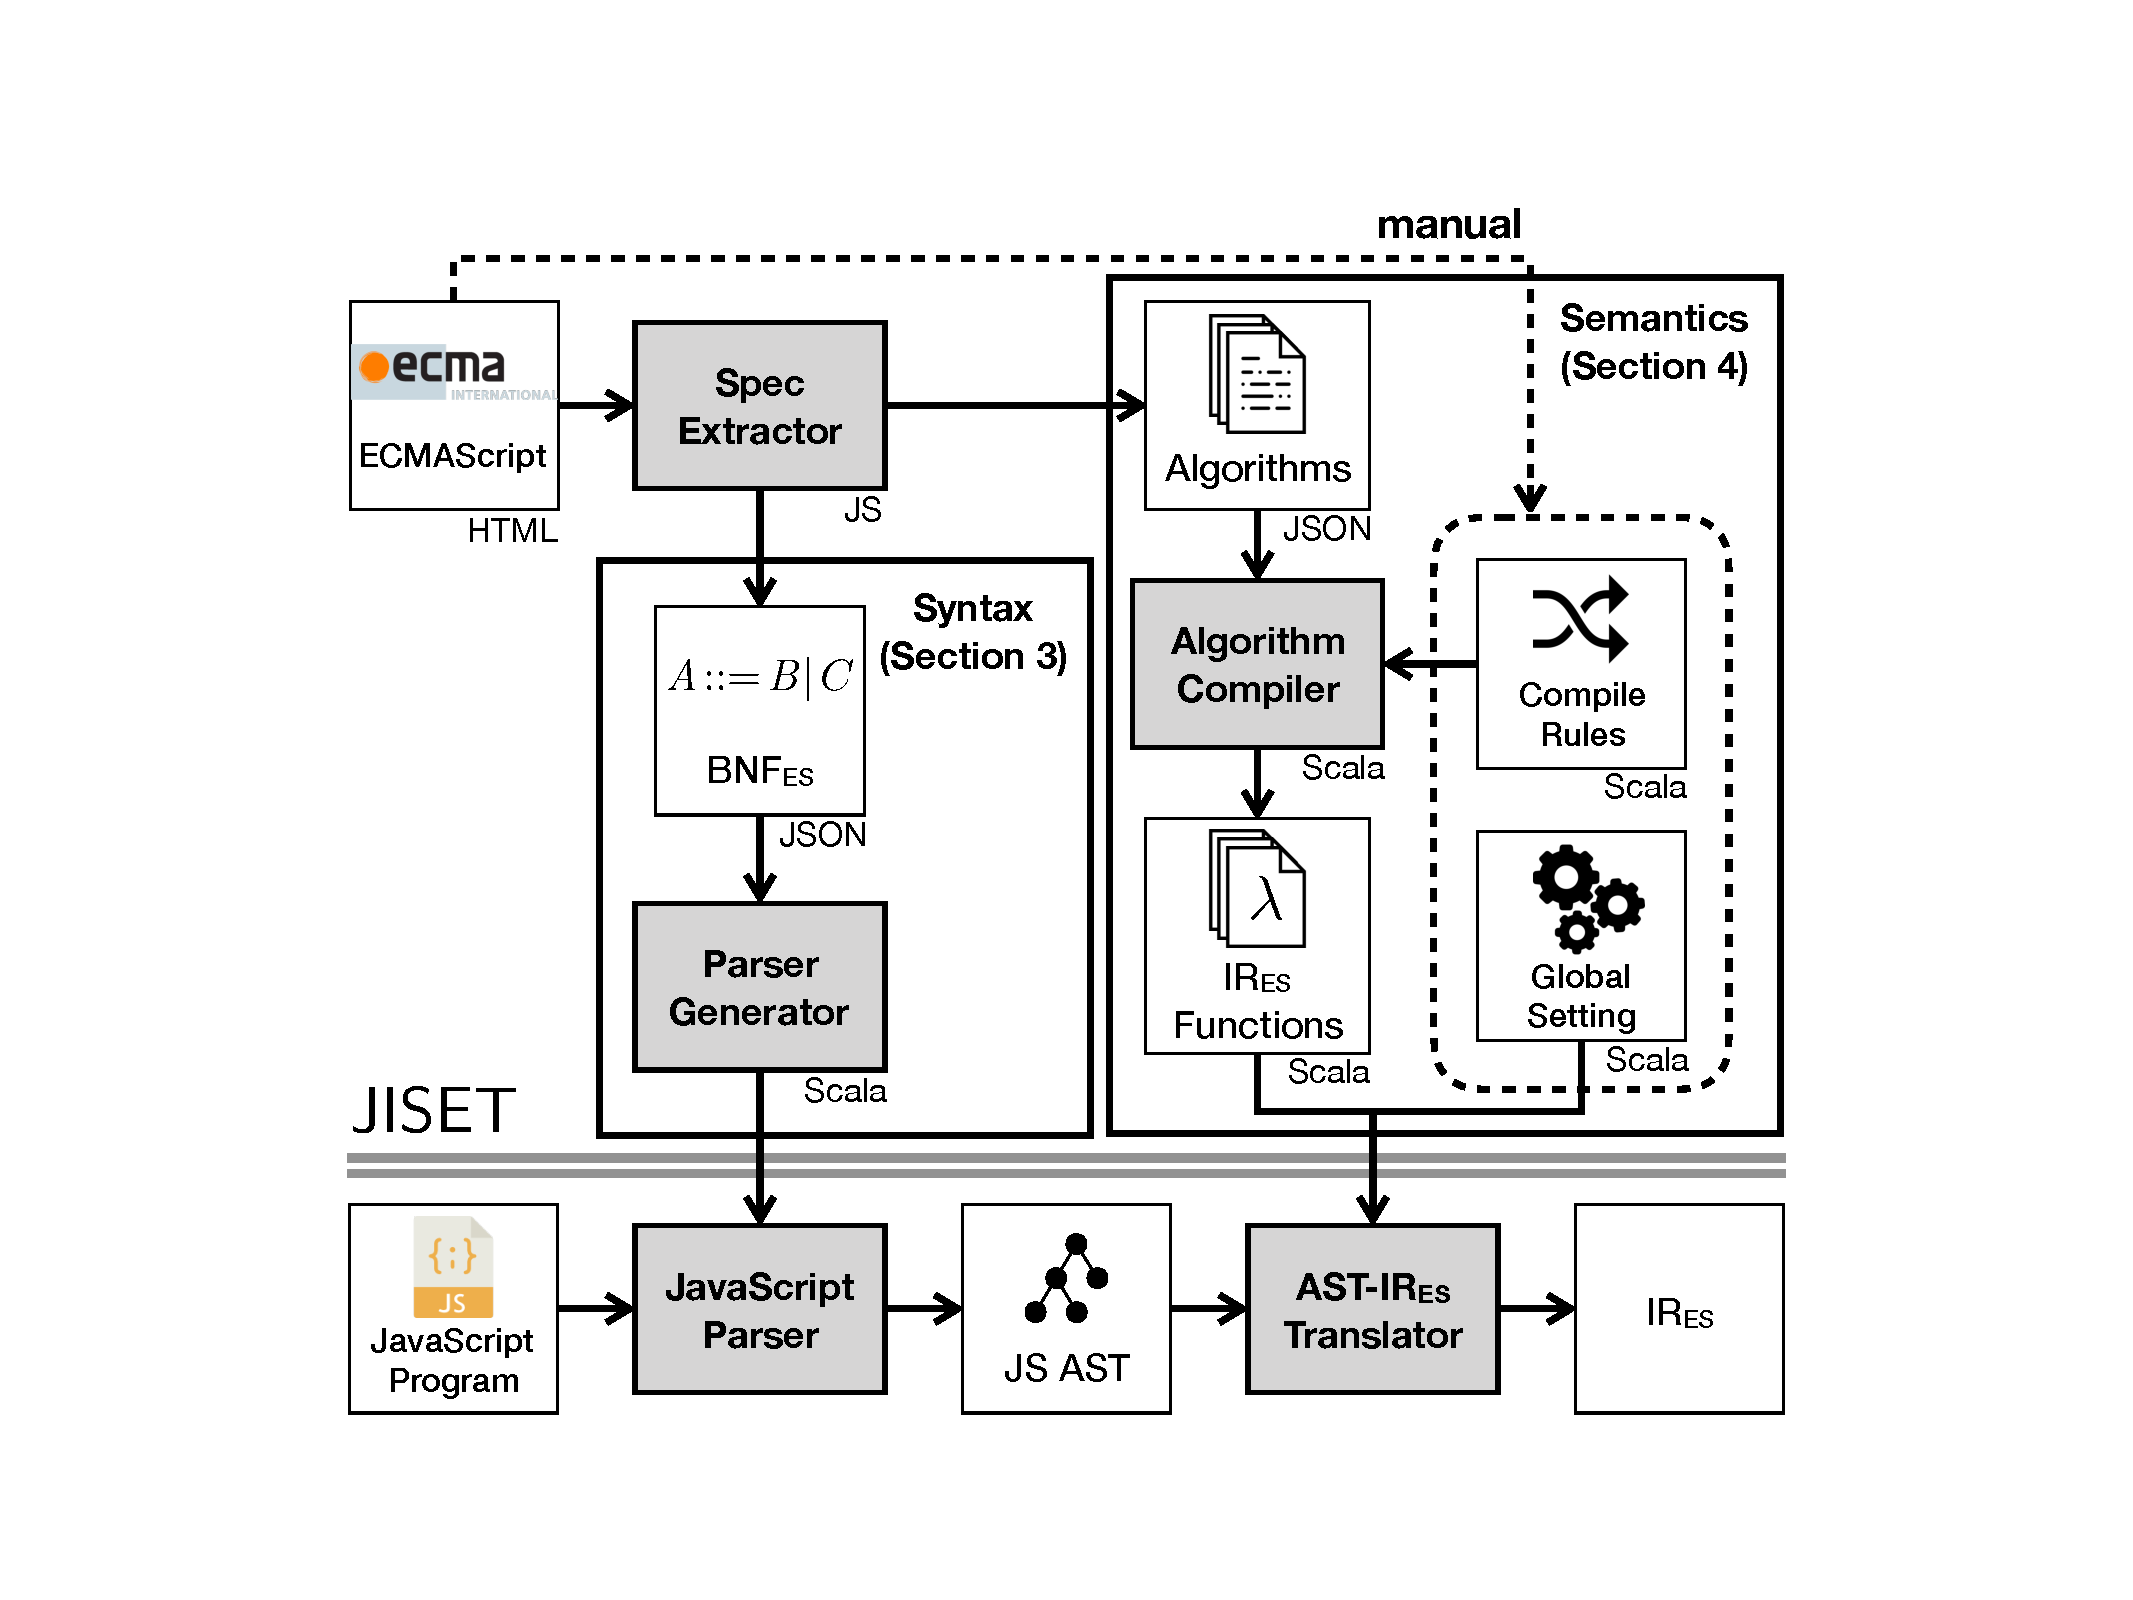
\includegraphics[width=0.48\textwidth]{img/overview.pdf}
  \caption{Overall structure of \( \tool \): Automatically synthesized {\sf
    JavaScript Parser} and {\sf AST-\( \ires \) Translator} for JavaScript
    IR-based semantics}
  \label{fig:overview}
\vspace*{-1em}
\end{figure}

In this section, we introduce the overall structure of \( \tool \) depicted in
Figure~\ref{fig:overview}.  Compared to the existing approaches shown in
Figure~\ref{fig:existing}, our tool automatically synthesizes {\sf JavaScript
Parser} and {\sf AST-\( \ires \) Translator} directly from ECMAScript. The
motivation of this work is twofold: 1) ECMAScript is written in a well-organized
style, and 2) the writing style is converged since ES7 in 2016.

We explain how \( \tool \) utilize such common patterns in the writing style to
synthesize two modules with an example.  After {\sf Spec Extractor} extract
syntax and semantics in JSON format, our tool consists consists of two parts for
\textit{syntax} and \textit{semantics}.

\begin{figure}
  \centering
  \begin{subfigure}[t]{0.4\textwidth}
    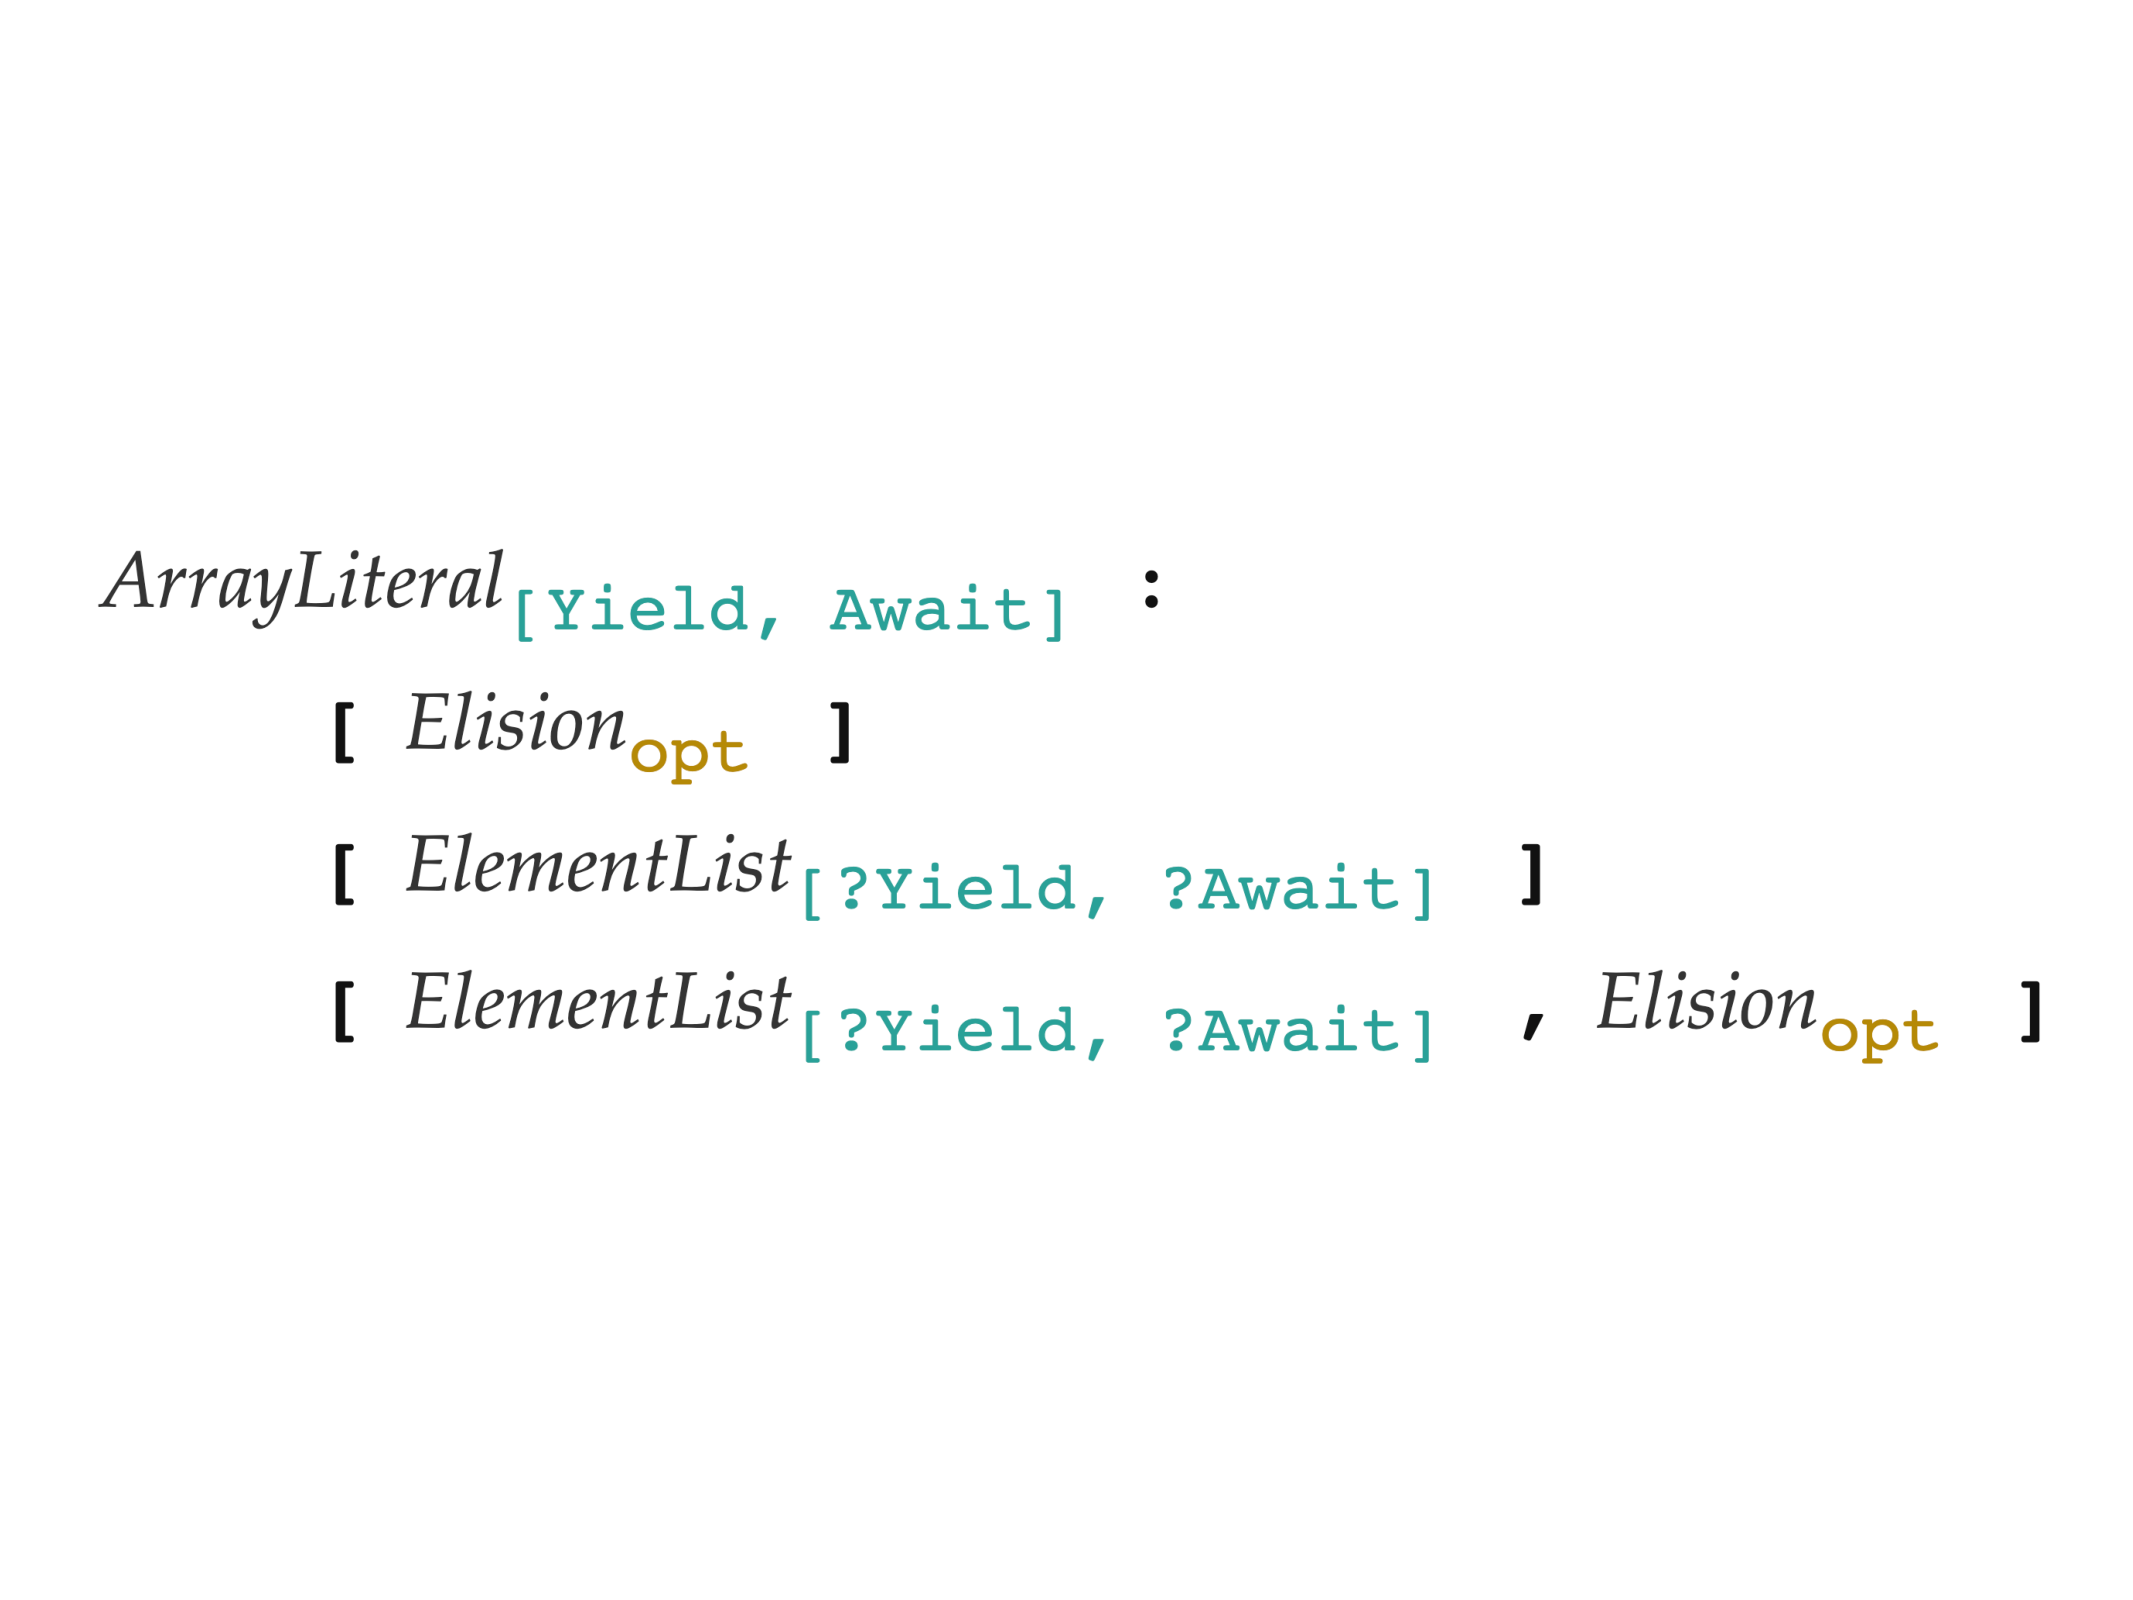
\includegraphics[width=\textwidth]{img/arrayliteral-syntax.pdf}
    \caption{\textit{ArrayLiteral} production in ES10}
    \label{fig:array-literal-es}
  \end{subfigure}
  \begin{subfigure}[t]{0.48\textwidth}
    \begin{lstlisting}[style=myScalastyle]
val ArrayLiteral: List[Boolean] => LAParser[T] = memo {
  case List(Yield, Await) =>
  "[" ~ opt(Elision) ~ "]"             ^^ ArrayLiteral0 |
  "[" ~ ElementList(Yield,Await) ~ "]" ^^ ArrayLiteral1 |
  "[" ~ ElementList(Yield,Await) ~ ","
      ~ opt(Elision)~ "]"              ^^ ArrayLiteral2
}
    \end{lstlisting}
    \vspace*{-1em}
    \caption{Generated parser for the \textit{ArrayLiteral} production}
    \label{fig:array-literal-parser}
  \end{subfigure}
  \vspace*{-1em}
  \caption{\textit{ArrayLiteral} production in ES10 and its parser}
  \label{fig:array-literal}
\end{figure}

\smallskip

\textbf{Syntax.} ECMAScript provides the lexical and syntactic grammars in
Appendix A using a variant of EBNF for ECMAScript.  We dub it \( \bnfes \) and
formally define it in Section~\ref{sec:parser}.  Our {\sf Spec Extractor} reads
the grammars written in \( \bnfes \) and converts them into JSON files.
For example, Figure~\ref{fig:array-literal}(a) shows the \textit{ArrayLiteral}
production in ES10.  It takes two boolean parameters \textsf{Yield} and
\textsf{Await} and has three alternatives.  The first alternative
consists of three symbols: two terminal symbols \( \code{[} \) and
\( \code{]} \), and one non-terminal symbol \textit{Elision}$_{\mbox{\footnotesize opt}}$.
The {\small opt} subscript denotes that it is optional.  In the second
and third alternatives, \textit{ElementList}$_{\mbox{\footnotesize\sf [?Yield, ?Await]}}$
denotes a parametric non-terminal symbol \textit{ElementList}
with the parameters \textsf{Yield} and \textsf{Await} of
\textit{ArrayLiteral} as its two arguments. The prefix \textsf{\small ?}
of a symbol denotes that the symbol is passed as an argument.

To generate {\sf JavaScript Parser} from a given \( \bnfes \) grammar, we
construct \textsf{Parser Generator} in Scala.  It synthesizes a
JavaScript parser according to the given \( \bnfes \), and the
generated parser is defined with Scala parser combinators~\cite{scala-parser-combinators}.
Moreover, in order to parse \( \bnfes \) grammars correctly and
efficiently, we propose \textit{lookahead parsers}, which keep track
of lookaheads, sets of possible next tokens.  With lookahead parsing,
generated parsers now have one-to-one mapping to their corresponding
grammar productions, improving readability.
For example, Figure~\ref{fig:array-literal}(b) shows the generated
parser for the \textit{ArrayLiteral} production in Figure~\ref{fig:array-literal}(a).
Each parser has the \( \code{List[Boolean] => LAParser[T]} \) type
because each production in \( \bnfes \) is parametric with boolean values.
The \( \code{memo} \) is a memoization function for pairs of boolean
parameters and resulting parsers for performance optimization.
The value \( \code{ArrayLiteral} \) corresponds to the
\textit{ArrayLiteral} production.  In the parser, each string literal
such as \( \code{"["} \) or \( \code{"]"} \) denotes a parser for a
terminal symbol.  The \( \code{opt} \) helper function creates
optional parsers.  The parametric non-terminal \textit{ElementList}
with arguments \textsf{Yield} and \textsf{Await} is represented as a
function call \( \code{ElementList(Yield, Await)} \).
The \( \code{\textasciitilde} \) operator combines two parsers
and the \( \code{\^{}\^{}} \) operator describes how to construct ASTs.
When the left-hand side of \( \code{\^{}\^{}} \) is matched, its
right-hand side shows a corresponding AST constructor, where the name
of each constructor has a number denoting the order among alternatives.
For example, the \( \code{ArrayLiteral0} \) constructor corresponds to
the first alternative of the \textit{ArrayLiteral} production.

\begin{figure}
  \centering
  \begin{subfigure}{0.43\textwidth}
    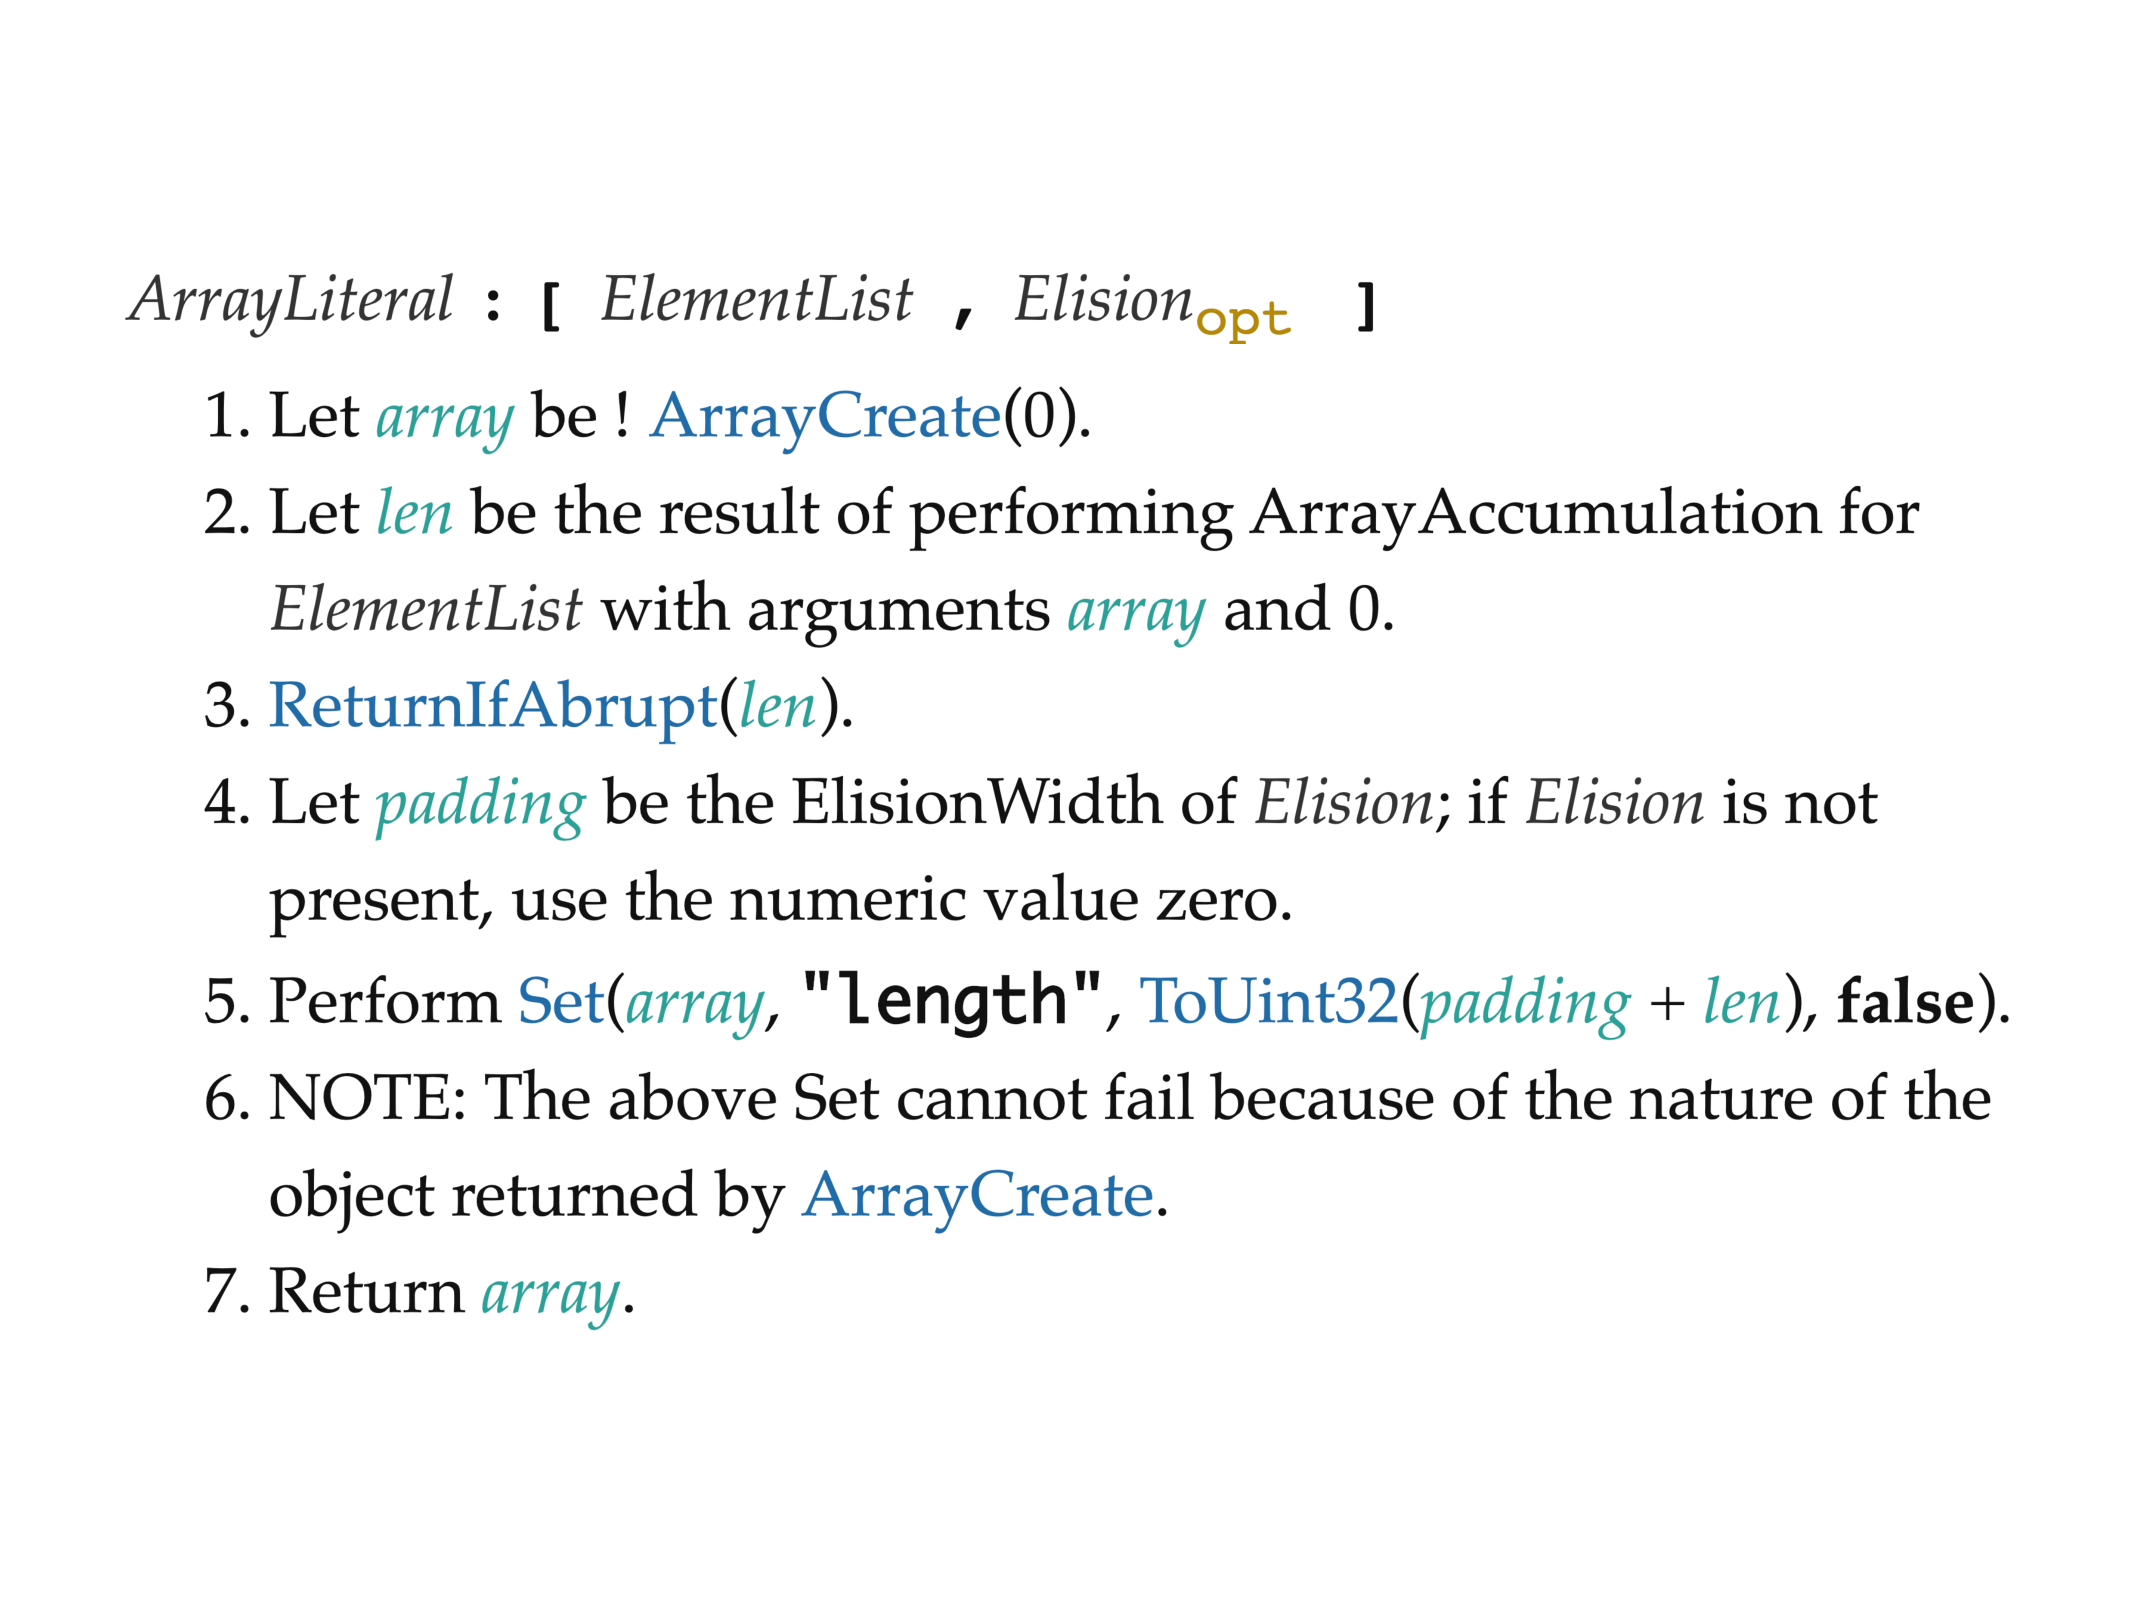
\includegraphics[width=\textwidth]{img/arrayliteral-eval.pdf}
    \subcaption{\textbf{Evaluation} abstract algorithm for the third alternative}
    \label{fig:array-literal-eval-es}
  \end{subfigure}
  \qquad
  \begin{subfigure}{0.46\textwidth}
    \begin{lstlisting}[style=ires]
ArrayLiteral[2].Evaluation (ElementList, Elision) => {
  let array = ! (ArrayCreate 0)
  let len = (ElementList.ArrayAccumulation array 0)
  ? len
  if (= Elision absent) let padding = 0
  else let padding = Elision.ElisionWidth
  (Set array "length" (ToUint32 (+ padding len)) false)
  return array
}
    \end{lstlisting}
    \vspace*{-1em}
    \subcaption{The generated \( \ires \) function}
    \label{fig:array-literal-eval-ires}
  \end{subfigure}
  \vspace{-1em}
  \caption{\textbf{Evaluation} abstract algorithm for the third alternative of
    \textit{ArrayLiteral} in ES10 and its generated \( \ires \)
    function}
  \label{fig:array-literal-eval}
  \vspace{-1em}
\end{figure}

\textbf{Semantics.}
ECMAScript describes the language semantics as abstract algorithms in English.
While they are written in a natural language, the writing style is
well-organized with ordered steps and tagged tokens.  {\sf Spec Extractor}
reads abstract algorithms with HTML tags and converts them into JSON files.
For example, Figure~\ref{fig:array-literal-eval}(a) presents the
\textbf{Evaluation} abstract algorithm of the third alternative of the
\textit{ArrayLiteral} production in ES10, and it has seven steps.  In the HTML
files describing the abstract algorithms, each non-terminal symbol
(e.g. \textit{ElementList}), local variable (e.g. \textit{array}), code (e.g. \(
\code{"length"} \)), or value (e.g. \textbf{false}) has the \( \code{<nt>} \),
\( \code{<var>} \), \( \code{<code>} \), or \( \code{<emu-val>} \) tag,
respectively.

To translate such abstract algorithms into representations
suitable for manipulation, we define \( \ires \), a specialized
intermediate representation for ECMAScript.  Then,
we develop \textsf{Algorithm Compiler} in Scala using Scala parser
combinators again to convert given abstract algorithms to \( \ires \)
functions.  It also takes \textsf{Compile Rules} as another input,
which has two parts: parsing rules and conversion rules.  They are
\textit{manually} specified for ECMAScript; we explain them in
detail in Section~\ref{sec:compiler}.  Thus, each abstract algorithm is
converted into a function written in \( \ires \) via \textsf{Algorithm Compiler}.
For example, Figure~\ref{fig:array-literal-eval}(b) presents the generated
\( \ires \) function for the \textbf{Evaluation} abstract algorithm shown in
Figure~\ref{fig:array-literal-eval}(a).
The \( \code{ArrayLiteral[2].Evaluation} \) function takes two parameters for
two non-terminal symbols: \( \code{ElementList} \) and \( \code{Elision} \).
The parameter \( \code{Elision} \) has a special value \( \code{absent} \) when
the non-terminal symbol \textit{Elision}$_{\mbox{\footnotesize opt}}$ is not
present.  Thus, we convert the condition in step 4,
``if \textit{Elision} is not present,'' into the equality check with \(
\code{absent} \): \( \code{if (= Elision absent)} \).  Codes are represented as
string values and values are represented as corresponding \( \ires \) values.
For instance, the code \texttt{\small "length"} and the value \textbf{false} are
converted into the string value \( \code{"length"} \) and the boolean value
\( \code{false} \), respectively.

Finally, \( \tool \) constructs {\sf AST-\( \ires \) Translator} with the given
\( \ires \) functions and \textit{manually} specified {\sf Global Setting},
which has minor but necessary information to evaluate JavaScript programs
described in ECMAScript such as the structure of the standard
built-in objects and ECMAScript data types. Putting them all together, we can
translate a given JavaScript program into \( \ires \) via generated {\sf
JavaScript Parser} and {\sf AST-\( \ires \) Translator} by \( \tool \).  Even
though \( \tool \) is not fully automatic because of {\sf Compile Rules} and
{\sf Global Setting}, it could dramatically reduce the efforts to building
parsers and translators from scratch.

In the remainder of this paper, we explain the details of how to
automatically generate parsers (Section~\ref{sec:parser}) and how to compile
abstract algorithms (Section~\ref{sec:compiler}).  After evaluating \( \tool \)
(Section~\ref{sec:eval}), we discuss related work (Section~\ref{sec:related}), and
conclude (Section~\ref{sec:conclude}).
